%
% Introduction to quantum information theory
%
\clearpage

\section{Introduction to quantum information theory}\index{Quantum information theory} \label{sec:quant_inf_th}

\famousquote{When you find yourself in a room surrounded by your enemies you tell yourself, `I am not locked in here with you, you are locked in here with me'. This is the kind of mindset you should have if you want to succeed in life. Get rid of that victim mentality.}{Bruce Lee}

\subsection{Probability, information \& classical correlation measures}

% The fundamental unit in Shannon information is the \textit{bit}. 

``Information theory begins with the observation that there is a fundamental link between probabilities and information'' \cite{barnett2009quantum}. 

Suppose that there are two parties trying to communicate, conventionally named Alice and Bob. Alice sends information using an alphabet $\{x_j \}$, and each letter occurs with probability $p_j$. If some letter occur less likely than others, then Bob will be more surprised receiving those, and one might naturally expect that the information content of those events are higher.

This suggests a way to measure the \textit{information content}\index{Information content} of an outcome, or how surprised Bob is,
\begin{align}
i(x_j) \equiv \log\left(\frac{1}{p(x_j)}  \right) =  -\log\left(p(x_j)  \right)
\end{align}

We can model Alice's source as a random variable $X$, whose outcomes are $\{ x_j\}$ each occurring with probability $p_j$. Then the expected information content of the source, or \textit{Shannon entropy}\index{Shannon entropy} associated with the $X$ is defined as,

\begin{align}\index{Shannon entropy}
H(X) = -\sum_i p_i\log_2(p_i).
\end{align}

Entropy plays a central role in information theory. The intuitive interpretation is that it quantifies an experimenter's uncertainty about $X$ before measuring it, and his expected information gain is $H(X)$ bits upon learning the outcome. The information $H(X)$ is zero if and only if one of the probabilities $p(x)$ is unity, with the others being zero. In this case the value of $X$ is already known and so there is no information to be gained from observing it.  

 If there are two random variables $X$ and $Y$, the joint entropy of the two is simply given by,
\begin{align}\index{Joint Shannon entropy}
H(X,Y) =  -\sum_{x,y} p_{x,y}\log_2(p_{x,y}).
\end{align}

Note that the joint entropy $H(X,Y)= H(X)+H(Y)$ if and only if $X$ and $Y$ are independent, i.e. the occurrence of one does not change the probability of the other.  

If the two distributions are not independent, i.e. knowing something about $X$ reveals information on $Y$, the two variables are said to be \textit{correlated}. Suppose Alice possesses the random variable $X$ and Bob has the random variable $Y$, the \textit{mutual information} specifies the number of bits in common between the two distributions. Equivalently, this represents the maximum number of bits that one party can learn about the other just by inspecting their own information.

For two classical distributions, the classical mutual information is given by,
\begin{align}\index{Mutual information}
I(X;Y) = H(X) + H(Y) - H(X,Y),
\label{eq:classical_mutual_info}
\end{align}
a measure of the correlation between the events $X$ and $Y$. The quantity in Eq.~\eqref{eq:classical_mutual_info} is important because it upper bounds the amount of information Alice and Bob can reliably communicate. For a discrete random variable with $d$ possible outcomes, the maximum mutual information between $X$ and $Y$ is $I(X,Y)=\log_2 d$ bits.

Another quantity of interest is the \textit{conditional entropy}, which describes the entropy of $Y$ should $X$ be known. The entropy of $Y$ conditioned on $X$ is given by,
\begin{align}
H(X|Y) &= H(X,Y)- H(Y) \nonumber\\
       &=- \sum_{x,y} p(x,y) \log_2 \frac{p(x,y)}{p(x)}.
\end{align}
Classically the conditional entropy is always positive, but as we will see later, this is not the case if quantum states are involved.

The relationship between the quantities mentioned above is graphically summarised in Fig.~\ref{fig:mutual_info}.

\begin{figure}[!htbp]
	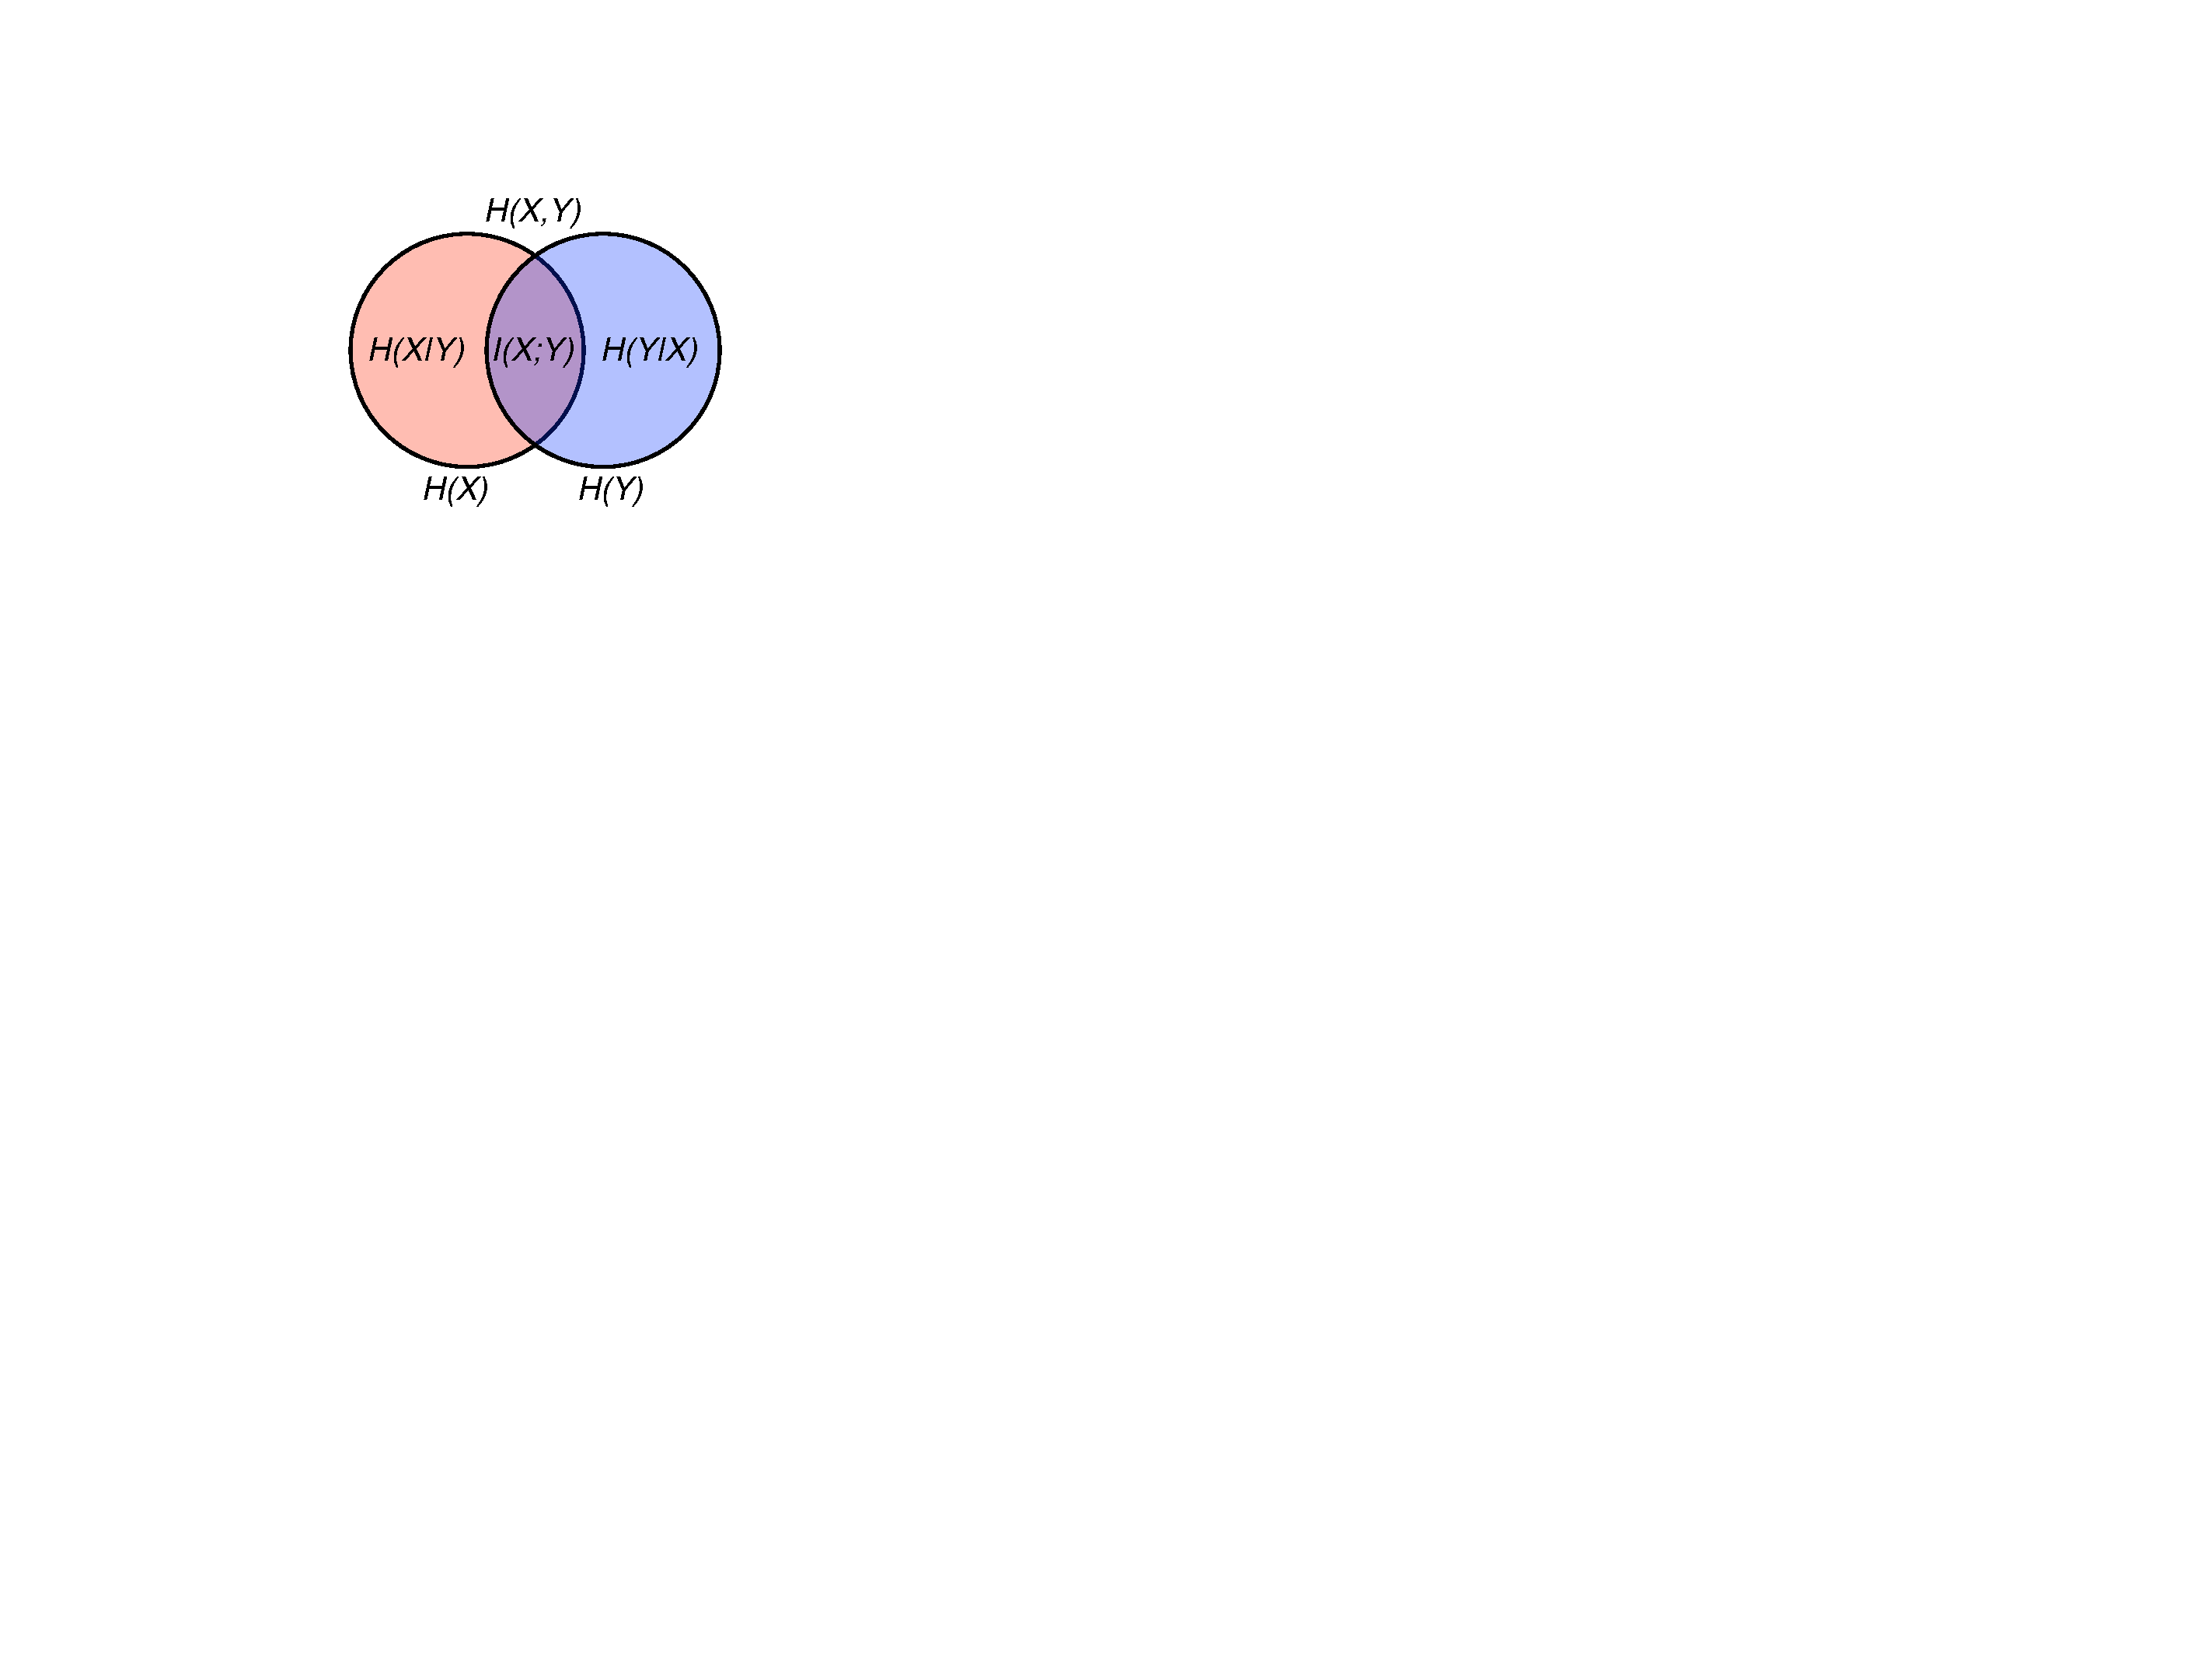
\includegraphics[clip=true, width=0.475\textwidth]{mutual_info}
	\captionspacefig \caption{Venn diagram showing the relationship between some elementary information theoretic entropy relations.} \label{fig:mutual_info}
\end{figure}

% 
% 
% 
% 
% 

\subsection{Quantum correlation measures}

The von Neuman entropy\index{von Neuman entropy} \cite{bib:bengtsson2017geometry} for quantum density operators, $S(\hat\rho)$, is defined analogously, replacing probabilities with density operator eigenvalues,
\begin{align}\index{von Neuman entropy}
S(\hat\rho) &= - \sum_x \lambda_x \log_2 (\lambda_x) \nonumber \\
&= -\mathrm{tr}(\hat\rho\,\log \,\hat\rho),
\end{align}
where $\{\lambda\}$ is the eigenvalue spectrum of $\hat\rho$. This modification is logically justified, as the eigenvalues can be interpreted directly as a purely classical probability distribution of orthogonal states when the density operator is transformed into a basis with no coherences between basis states (i.e a diagonal basis or spectral decomposition\index{Spectral decomposition}). In that case, the Shannon and von Neuman entropies essentially have identical physical interpretations.

There are a few properties of the von Neumann entropy which are often usefuL:
\begin{enumerate}
	\item For pure states $\hat \rho = \ket{\psi}\bra{\psi}$,
		\begin{align}
			S(\hat\rho) = 0.
		\end{align}
	\item The von Neumann entropy is invariant under change of basis transformations (i.e conjugation by a unitary operator), 
			\begin{align}
			S(U\hat \rho U^\dagger) = S(\hat \rho)
			\end{align}
	\item For a state living in a Hilbert space of dimension $d$,
		\begin{align}
			S(\hat\rho) \leq \log_2 d,
		\end{align}
	with equality being achieved when the quantum state is maximally mixed.
	\item For a given bipartite system $AB$,
			\begin{align}
			S(\hat \rho_{AB}) \leq S(\hat \rho_A) + S(\hat \rho_B),
			\end{align}
			where equality holds if $\hat\rho_{AB}= \hat\rho_A \otimes \hat\rho_B$.
\end{enumerate}

Analogously, the quantum mutual information\index{Quantum mutual information} for bipartite state $\hat\rho_{A,B}$ is defined as,
\begin{align}
I(A;B)_{\hat\rho} = S(\hat\rho_A) + S(\hat\rho_B) - S(\hat\rho_{A,B}),
\end{align}
using the von Neuman entropy.

The mutual information between two quantum states is invariant under local unitary transformation,
\begin{align}
I(A;B)_{\hat\rho} = I(\hat{U}_A\hat\rho_A \hat{U}_A^\dag; \hat{U}_B\hat\rho_B \hat{U}_B^\dag),
\end{align}
since the eigenvalue spectrum of a density operator is invariant under unitary transformations. Therefore, the mutual information represents the maximum amount of information Bob can learn about Alice's state under \textit{any} local operations.

Now, in sharp contrast with the classical case, the conditional entropy for quantum states,
\begin{align} \label{cond_quant_ent}
H(A| B)_{\hat \rho} = S(\hat \rho_{AB}) - S(\hat \rho_B),
\end{align}
can be negative! If $\hat\rho_{AB}$ is a maximally entangled state, then $S(\hat \rho_{AB}) =0$, and $H(A|B) =- S(\hat \rho_{AB}) <0$. Intuitively, this can be interpreted as the fact that bipartite maximally entangled states can be more strongly correlated than classically possible, and that knowing the state of $A$ reveals an `unnatural' amount of information about the state of $B$.

A quantum process cannot increase the mutual information between two parties. This yields the \textit{data processing inequality}\index{Data processing inequality} that, for a sequence of channels \mbox{$X\to Y\to Z$},
\begin{align}\index{Data processing inequality}\label{eq:data_proc_ineq}
I(X:Z)&\leq I(X:Y), \nonumber \\
I(X:Z)&\leq I(Y:Z),
\end{align}
with equality if and only if the channel not specified in the identity on the right hand side (\mbox{$Y\to Z$} or \mbox{$X\to Y$} respectively) is unitary, i.e one of the links in the chain perfectly preserves information content. The progression is shown in Fig.~\ref{fig:data_proc_ineq}.

\begin{figure}[!htbp]
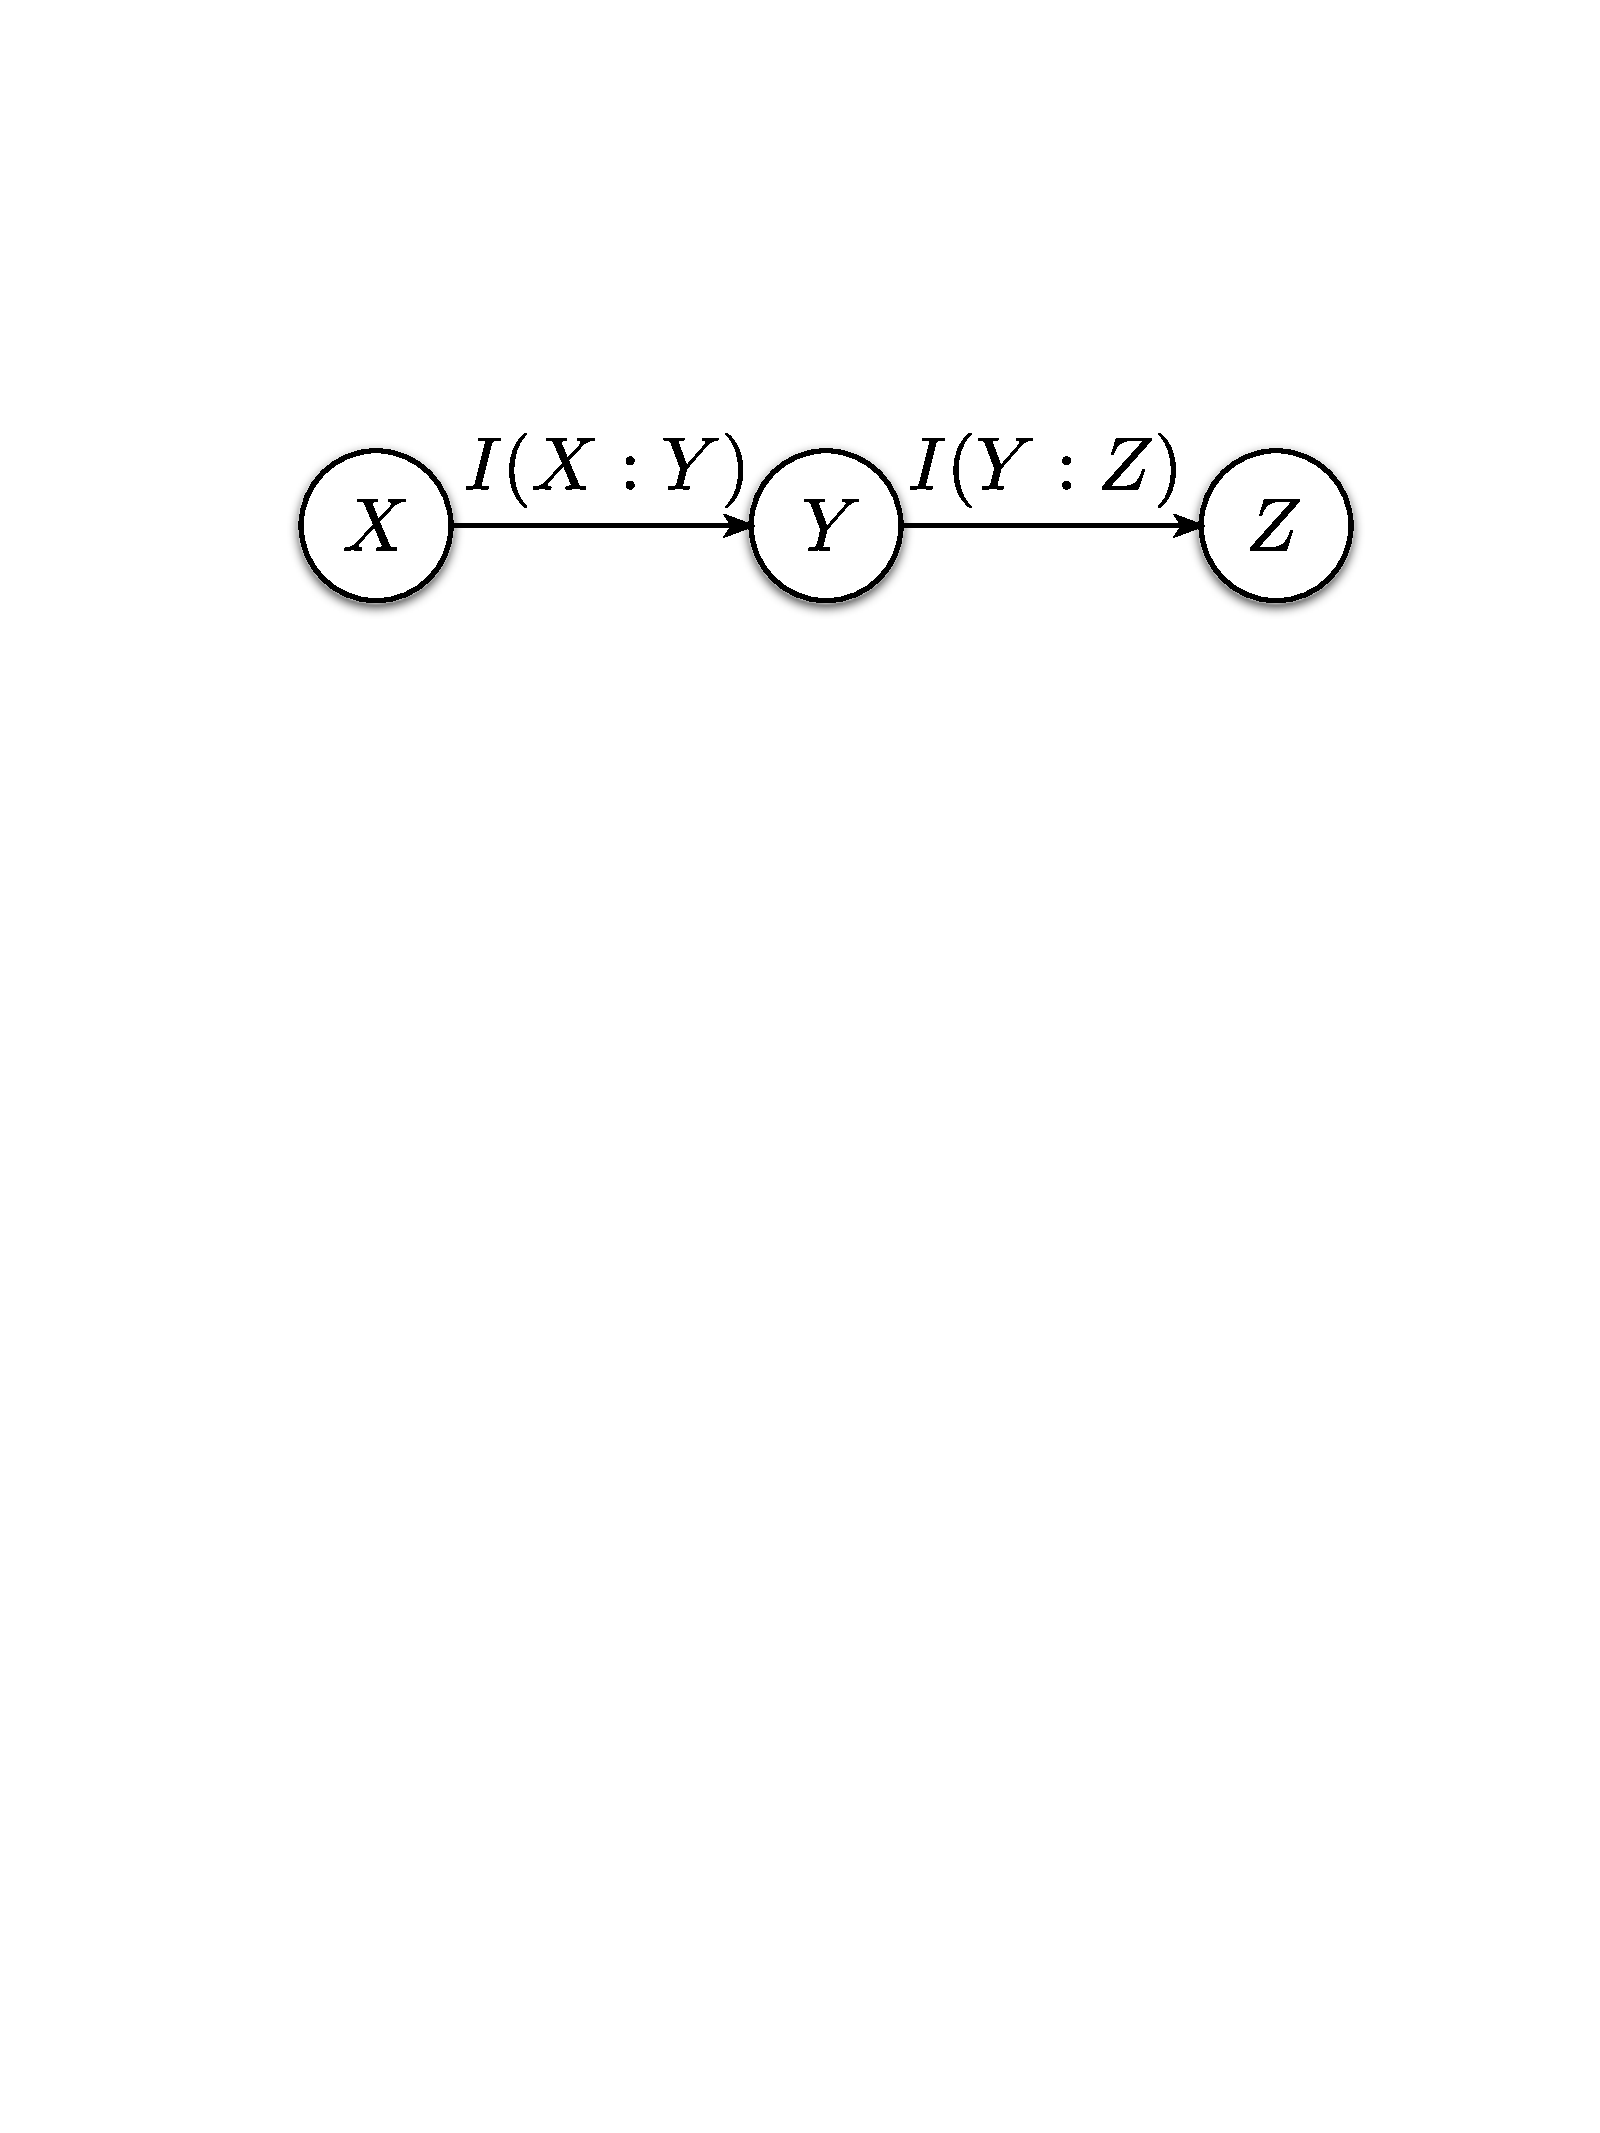
\includegraphics[clip=true, width=0.3\textwidth]{data_proc_ineq}
\captionspacefig \caption{\label{fig:data_proc_ineq}A sequence of events \mbox{$X\to Y\to Z$}. The data processing inequality states that the mutual information from beginning to end is upper-bounded by the mutual information between neighbouring stages, as per Eq.~(\ref{eq:data_proc_ineq}).}	
\end{figure}

The mutual information is defined as being between a particular known pair of states. Of course, in a quantum channel we have the flexibility to manipulate the input state and the measurement at the output. From this, we can then define the \textit{classical information of the channel}\index{Classical information of the channel}, $I_c(\hat\rho_{A,B})$ --- the maximum of the mutual information, optimised over \textit{all} possible measurement settings. Suppose $\hat\rho_{A,B}$ is shared between Alice and Bob, from which they would like to extract maximal correlations (i.e joint information). They measure using local measurement bases $\{\Lambda_A^x\}$ and $\{\Lambda_B^x\}$, yielding random variables $A$ and $B$. The quantum mutual information of the channel $\mathcal{E}$ is defined as,
\begin{align} \label{eq:channel_quant_mutual}
I_c(\mathcal{E}) = \max_{\rho,\{\Lambda_A^x\},\{\Lambda_B^x\}} I(A;B)_\rho. 
\end{align}

Eq.~\eqref{eq:channel_quant_mutual} quantifies the maximum amount of correlation that can be established between input and output states that can be achieved across the channel. This dictates the physical upper bound on the achievable bitrate (classical communication) or bandwidth of the channel.

All of the correlations discussed above concern classical information. Whilst classical correlation measures have a clear operational meaning, quantum channel capacities less so --- these quantities can be interpreted as how well the channel preserves the quantum state.

That the conditional entropy for quantum states can be negative is significant. In fact, it has its own name and notation, the \textit{coherent information},
\begin{align}
I(A\rangle B) = H(B)_{\hat\rho} - H(A,B)_{\hat\rho},
\end{align}
For a maximally entangled state, the coherent information is equal to one. It measures to what extent we know less about a subsystem compared to the whole.

%
% Channel Capacity
%

\subsection{Channel capacity} \label{sec:channel_cap} \index{Channels!Capacity}

The measures considered until now have quantified the preservation of quantum states. Alternately, one might consider information theoretic measures\index{Information theoretic!Measures}, which quantify the number of bits/qubits transmitted by a link, i.e the number of bits/qubits in common before and after the channel. This is an extremely powerful tool as it upper bounds the amount of information the receiver can extract from the transmitter under \textit{any} measurement scheme, very useful in a cryptographic context, where we want security to be attack-independent\index{Information-theoretic!Security} (Sec.~\ref{sec:comp_vs_inf_th_sec}). 



% Before we delve into this, we have to introduce a few new quantities.

% \paragraph{Classical correlation measures}

% Suppose we have a random variable $X$, and a particular measurement outcome $x$ occurs with probability $p(x)$, the Shannon entropy of $X$ is given by,
% \begin{align}\index{Shannon entropy}
% H(X) = -\sum_x p_x\log_2(p_x).
% \end{align}

% The information, or entropy, plays a central role in information theory. The intuitive interpretation is that it quantifies an experimenter's uncertainty about $X$ before measuring it, and his expected information gain is $H(X)$ bits upon learning the outcome. The information $H(X)$ is zero if and only if one of the probabilities $p(x)$ is unity, with the others being zero. In this case the value of $X$ is already known and so there is no information to be gained from observing it.  

%  For a joint distribution over $X$ and $Y$ this simply generalises to,
% \begin{align}\index{Joint Shannon entropy}
% H(X,Y) =  -\sum_{x,y} p_{x,y}\log_2(p_{x,y}).
% \end{align}

% The von Neuman entropy\index{von Neuman entropy} \cite{bib:bengtsson2017geometry} for quantum density operators, $S(\hat\rho)$, is defined analogously, replacing probabilities with density operator eigenvalues,
% \begin{align}\index{von Neuman entropy}
% S(\hat\rho) &= - \sum_x \lambda_x \log_2 (\lambda_x) \nonumber \\
% &= -\mathrm{tr}(\hat\rho\,\log \,\hat\rho),
% \end{align}
% where $\{\lambda\}$ is the eigenvalue spectrum of $\hat\rho$. This modification is logically justified, as the eigenvalues can be interpreted directly as a purely classical probability distribution of orthogonal states when the density operator is transformed into a basis with no coherences between basis states (i.e a diagonal basis or spectral decomposition\index{Spectral decomposition}). In that case, the Shannon and von Neuman entropies essentially have identical physical interpretations.

% We now introduce an entropic measure of common or mutual information shared by two parties. Suppose Alice possesses the random variable $A$ and Bob has the random variable $B$, the \textit{mutual information} specifies the number of bits in common between the two distributions. Equivalently, this represents the maximum number of bits that one party can learn about the other just by inspecting their own information.

% For two classical distributions, the classical mutual information is given by,
% \begin{align}\index{Mutual information}
% I(A;B) = H(A) + H(B) - H(A,B).
% \end{align}
% Analogously, the quantum mutual information\index{Quantum mutual information} for bipartite state $\hat\rho_{A,B}$ is defined as,
% \begin{align}
% I(A;B)_{\hat\rho} = S(\hat\rho_A) + S(\hat\rho_B) - S(\hat\rho_{A,B}),
% \end{align}
% using the von Neuman entropy.

% The mutual information between two quantum states is invariant under local unitary transformations,
% \begin{align}
% I(A;B)_{\hat\rho} = I(\hat{U}_A\hat\rho_A \hat{U}_A^\dag; \hat{U}_B\hat\rho_B \hat{U}_B^\dag),
% \end{align}
% since the eigenvalue spectrum of a density operator is invariant under unitary transformations. Therefore, the mutual information represents the maximum amount of information Bob can learn about Alice's state under \textit{any} local operations.

% A quantum process cannot increase the mutual information between two parties. This yields the \textit{data processing inequality}\index{Data processing inequality} that, for a sequence of channels \mbox{$X\to Y\to Z$},
% \begin{align}\index{Data processing inequality}\label{eq:data_proc_ineq}
% I(X:Z)&\leq I(X:Y), \nonumber \\
% I(X:Z)&\leq I(Y:Z),
% \end{align}
% with equality if and only if the channel not specified in the identity on the right hand side (\mbox{$Y\to Z$} or \mbox{$X\to Y$} respectively) is unitary, i.e one of the links in the chain perfectly preserves information content. The progression is shown in Fig.~\ref{fig:data_proc_ineq}.

% \begin{figure}[!htbp]
% 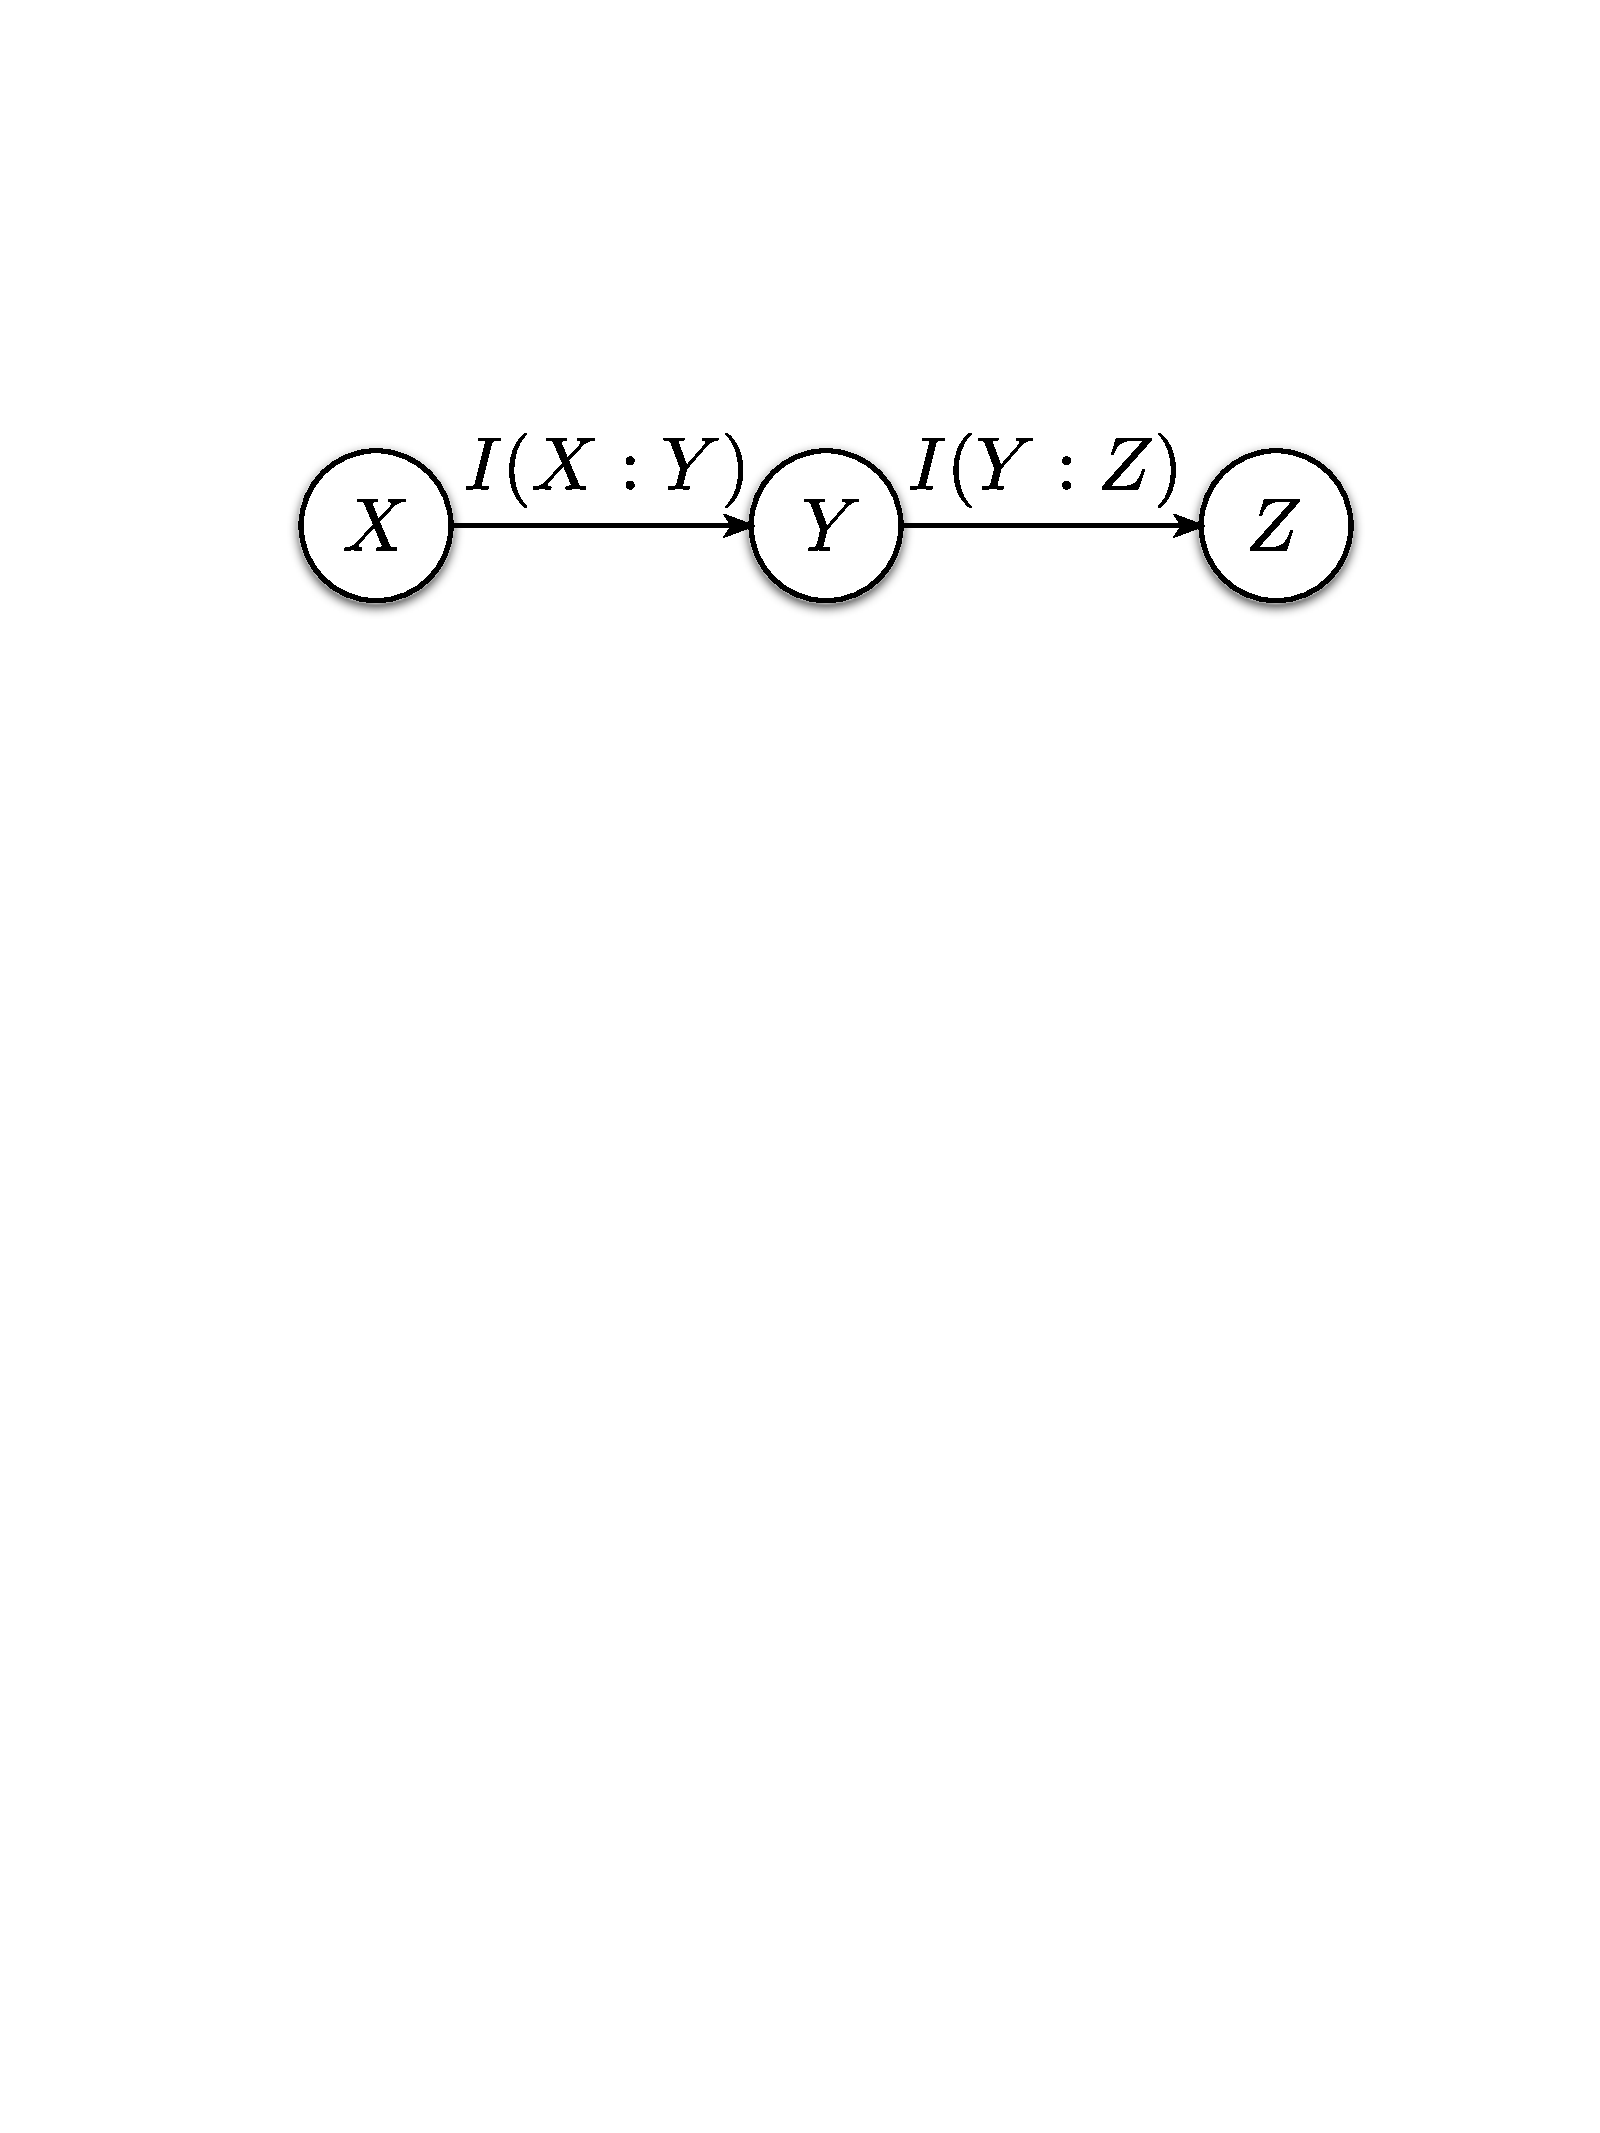
\includegraphics[clip=true, width=0.3\textwidth]{data_proc_ineq}
% \captionspacefig \caption{\label{fig:data_proc_ineq}A sequence of events \mbox{$X\to Y\to Z$}. The data processing inequality states that the mutual information from beginning to end is upper-bounded by the mutual information between neighbouring stages, as per Eq.~(\ref{eq:data_proc_ineq}).}	
% \end{figure}

% The mutual information is defined as being between a particular known pair of states. Of course, in a quantum channel we have the flexibility to manipulate the input state and the measurement at the output. From this, we can then define the \textit{classical information of the channel}\index{Classical information of the channel}, $I_c(\hat\rho_{A,B})$ -- the maximum of the mutual information, optimised over \textit{all} possible measurement settings. 

Suppose $\hat\rho_{A,B}$ is shared between Alice and Bob, from which they would like to extract maximal correlations (i.e joint information). They measure using local measurement bases $\{\Lambda_A^x\}$ and $\{\Lambda_B^x\}$, yielding random variables $A$ and $B$. Recall from Sec.~\ref{sec:quant_inf_th} that the quantum mutual information of the channel is defined as,

\begin{align} \label{eq:quant_mut}
I_c(\hat\rho_{A,B}) = \max_{\rho,\{\Lambda_A^x\},\{\Lambda_B^x\}} I(A;B).
\end{align}

The intuitive interpretation is that this is the maximum mutual information between input and output states that can be achieved across the channel. This effectively places a physical upper bound on the achievable bitrate or bandwidth of the channel.

\noindent We are then led to the definition of the \textit{classical channel capacity} of a quantum channel $\mathcal{E}$,
\begin{align}\index{Classical!Channels!Capacity}
\mathcal{C}(\mathcal{E}) = \lim_{n \rightarrow \infty} \frac{I_c(\mathcal{E}^{\otimes n})}{n},
\end{align}
which can be interpreted as the maximum bitrate of the channel, per use of the channel, in the limit of an infinite number of uses, where entangled between multiple applications is allowed in general.

 For a noisy channel, if the input contains product states as well as separable measurements, the classical capacity is equal to Eq.~(\ref{eq:quant_mut}), that is, the single-use and the asymptotic classical capacities are equal.

If we also allow joint measurement (but not entanglement between input states), the classical channel capacity can be expressed as,
\begin{align}
\chi(\mathcal{E}) = \max_{p_i,\hat\rho_i} S(\hat\rho) - \sum_i p_i S(\hat\rho_i), \label{eq:holevoinfo}
\end{align}
known as the Holevo bound\index{Holevo bound}\index{Holevo bound}.

However, if entangled input states are allowed in conjunction with joint measurement setting, the Holevo bound no longer holds, and the asymptotic classical channel capacity,
\begin{align}
\chi(\mathcal{E}) < \mathcal{C(E)}.
\end{align}

It has been shown that using entangled input states in conjunction with joint measurements can increase the amount of classical information which can be transmitted over a noisy quantum channel. In this case, 
\begin{align}
C_\text{ent} = \lim _{n\to \infty} \frac{1}{n}\chi(\mathcal{E}^{\otimes n}).
\label{eq:ent_ent}
\end{align}

The private classical capacity\index{Private channel capacity} $\mathcal{P(E)}$ of a quantum channel $\mathcal{E}$ describes the maximum rate at which the channel is able to send classical information through the channel reliably and privately, that is, the trusted parties do not want the environment to have access to their classical correlations.

Here Alice prepares the quantum state $\hat\rho_x^A$ according to the probability distribution $\{p_X(x)\}$. The expected density operator of the ensemble is of the form,
\begin{align}
\hat\rho^{XA} \equiv \sum_x p_X(x)\ket{x}\bra{x}  \otimes p_x^A.
\end{align}

The difference between the amount of classical correlation that she can establish with Bob, minus the correlation obtainable by Eve is given by,
\begin{align}
I(X;B)_\rho - I(X;E)_\rho,
\end{align}
which leads to the definition of the \textit{private information of a quantum channel}, where Alice maximises over all of her inputs,
\begin{align}
I_\mathcal{P} = \max_{\rho^{XA}} \{I(X;B)_\rho - I(X;E)_\rho \}.
\end{align}

The private classical capacity is defined as,
\begin{align}
\mathcal{P(E)} = \lim_{n\rightarrow \infty} \frac{1}{n} I_\mathcal{P}(\mathcal{E}^{\otimes n })
\end{align}

The last capacity in regards to classical communication over quantum channel is the \textit{entanglement-assisted classical capacity}\index{Entanglement-assisted classical capacity}, $\mathcal{C}_E(\mathcal{E})$. This quantity measures the classical information that can be transmitted through the channel, if Alice and Bob possess shared entanglement prior to the transmission,
\begin{align}
\mathcal{C}_E(\mathcal{E}) = \max_{p_i,\hat\rho_i} I(A:B).
\end{align}

The difference between $\mathcal{C(E)}$ and $\mathcal{C}_E(\mathcal{E}) $ is that $\mathcal{C}_E(\mathcal{E}) $ is equal to the maximised quantum mutual information (i.e additivity holds), and is equal to the single-use version of $\mathcal{C}_E(\mathcal{E})$. This implies that shared entanglement does not change the additivity of quantum mutual information.

\subsection{Quantum channel capacity}

The quantum coherent information exhibits much of the same mathematical structure as the classical mutual information. And analogously,
\begin{align}\index{Quantum channels!Capacity}
\mathcal{I}_Q(\mathcal{E}) = \max_{\hat\rho} I_\text{coh}(\hat\rho,\mathcal{E}).
\label{eq:mutual_info_quantum_single}
\end{align}

The \textit{quantum channel capacity}\index{Quantum channel capacity} is then analogously defined as,
\begin{align}\label{eq:quantcohinfo}
Q(\mathcal{E}) = \lim_{n \rightarrow \infty} \frac{\mathcal{I}_Q(\mathcal{E}^{\otimes n})}{n}.
\end{align}

The most important distinction between quantum mutual information and quantum coherent information is that the mutual information is always additive, but the quantum coherent information is not.

Analytic solutions to Eq.~(\ref{eq:quantcohinfo}) are notoriously difficult to calculate. However, once net dephasing or depolarisation rates have been calculated across a route, the \textit{single-use} quantities can be calculated, which can serve as a lower bound to the ultimately achievable rates, if a number representing \textit{cost}, rather than an analytic solution, is all we need.

A summary of the different measure of classical and quantum capacities are given in Tab.~\ref{tab:capacities}.

\startnormtable
\begin{table*}[!htbp]
\begin{tabular}{ |c | c | c| c| } \hline
Capacity & Type of information & Correlation measure &Capacity formula  \\ \hline
Classical &Classical information &Holevo information &Eq.~(\ref{eq:holevoinfo})       \\
Private & Classical information & Private information  & See \cite{bib:PhysRevLett.103.120501} \\
Entanglement-assisted classical & Classical information & Quantum mutual information & See \cite{bib:PhysRevLett.83.3081} \\
Quantum &Quantum information &Quantum coherent Information &Eq.~(\ref{eq:quantcohinfo}) \\ \hline
\end{tabular}
\captionspacetab
\caption{\label{tab:capacities} Measure of classical and quantum channel capacities. Taken from \cite{bib:8242350}.}
\end{table*}
\startalgtable

We now discuss the quantum capacity for the erasure channel and the amplitude damping channel, both of which the quantum capacities can be calculated.

The erasure channel acts on a state as follows is,
\begin{align}
\hat\rho \rightarrow (1-\eta) \hat\rho + \eta\ket{e}\bra{e}
\end{align}
where $\eta$ is the probability of losing the state and $\ket{e}\bra{e}$ is orthogonal to $\rho$. Given a system of dimension $d_A$, For $\eta \in [1/2,1]$, the quantum capacity is zero. For $\eta \in [0,1/2]$, the quantum capacity is $(1-2\eta)\log d_A.$

For an amplitude damping channel with damping parameter $\gamma$, the Kraus operators can be written as,
\begin{align}
A_0 &= \ket{0}\bra{0} + \sqrt{1-\gamma}\ket{1}\bra{1},\nonumber\\
A_1 &= \sqrt{\gamma}\ket{1}\bra{1}.
\end{align}

For $\gamma \in [0,1/2]$,the quantum capacity is equal to,
\begin{align}
\max_{p \in [0,1]} h_2 [(1-\gamma)p] - h_2[\gamma_p],
\end{align}
where $h_2$ represents the binary entropy function. For $\gamma \in [1/2,1]$, the quantum capacity is equal to zero.

Two of the most surprising discoveries of quantum Shannon theory is the \textit{superadditivity}\index{Superadditivity} of coherent information for the depolarising channel, and \textit{superactivation} of quantum capacity, where two channels whose individual capacities are zero can be combined to make a channel with non-zero capacity.

\subsection{Superadditivity of coherent information}

For qubits, the depolarising channel transmits its input with probability $(1-p)$ and replaces it with the maximally mixed state $\hat\openone/2$ with probability $p$,
\begin{align}
\rho \rightarrow (1-p) \rho + p \frac{\openone}{2}.
\end{align}
It is known that its coherent information is strictly superadditive when $p$ is large.

\begin{align}
I_\mathcal{Q}(\mathcal{E}) < 5 I_\mathcal{Q}(\mathcal{E}^{\otimes 5}).
\end{align}

It can be shown that the state which maximises the coherent information is the Bell state $\frac{1}{\sqrt2}(\ket{00}_{AA_1} + \ket{11}_{AA_1} )$, and the one-use coherent information is,
\begin{align} \label{eq:qcohdepol}
I_\mathcal{Q} = 1+ \left( 1-\frac{3p}{4} \right )\log\left[1-\frac{3p}{4}\right] + \frac{3p}{4}\log\left[\frac{p}{4}\right].
\end{align}

At $p = 0.25$, Eq.~\eqref{eq:qcohdepol} is equal to zero, but if we calculate the coherent information for a five-qubit repetition code,
\begin{align}
\frac{1}{\sqrt2}&(\ket{00}_{AA_1} + \ket{11}_{AA_1} ) \rightarrow \nonumber \\ 
\frac{1}{\sqrt2}&(\ket{000000}_{AA_1A_2 A_3 A_4 A_5} + \ket{111111}_{AA_1A_2 A_3 A_4 A_5}),
\end{align}
at $p$ just above $0.25$, the quantity of interest is positive \cite{bib:PhysRevA.57.830}. This demonstrates that the quantum capacity of the depolarising channel is superadditive. Despite the fact that the channel looks simple, the best strategy for achieving the quantum capacity of the depolarising channel remains very poorly understood \cite{bib:wilde2013quantum}.

\subsection{Superactivation}\index{Superactivation}

Suppose that Alice is connected to Bob by two quantum channel $\mathcal{E}_1,\mathcal{E}_2$ both with zero quantum capacity. Intuitively one would expect that Alice would not be able to transmit quantum information over the channel $\mathcal{E}_1\otimes \mathcal{E}_2$. However, examples of two zero-capacity channels are known to have non-zero joint quantum capacity. The phenomenon is known as \textit{superactivation}.

One of the channels is a 50\% erasure channel (which we know to have zero quantum capacity from the non-cloning theorem), and the other is known as an entanglement-binding channel \cite{bib:horodecki2001separability}.

This phenomenon has important implications for quantum information transmission. It implies that if there are other seemingly useless channels available, one could transmit more quantum information than if the channels were used alone. It also implies that the coherent information is strongly non-additive, and there is much to be understood about reliable communication rates over quantum channels.
